\documentclass[12pt]{article}

\usepackage[left= 2.5cm, right= 2.5cm, top= 2cm, bottom= 2cm]{geometry}

\usepackage[spanish]{label}

\usepackage{graphix}

\usepackage{amsmath, amsthm, amssymb, amsfonts}

\usepackage{hyperref}

\usepackage{listings}
\lstset{language=Python}

%Document

\title{\Huge Prácticum \LaTeX}
\author{\Large Manuel Mateo Delgado-Gambino López}
\date{10/03/2023}

\begin{document}

    \maketitle

    \clearpage

    \tableofcontents

    \clearpage

    \section{Ejercicio_1}

      Considera la ecuación:

      \begin{equation}\label{Polinomio}
        x^5-5x+1=0
      \end{equation}
         
      1.1.Haz un análisis de la función f(x)= \eqref{Polinomio}, obteniendo intervalos de monotonía, extremos relativos, límites cuando x->+$\infty$ o x->-$\infty$, etc.
      1.2.Basándote en dicho estudio y en la gráfica de la función f, justifica analiticamente cuántas soluciones tiene la ecuación del enunciado y en qué intervalos se localizan, apoyándote para ello en un teorema conocido.
      1.3.Utiliza el método de dicotomía para aproximar las raíces de la ecuación anterior con un error < $10^{-8}$ y comparte el código en Python que has utilizado para ello.
      1.4.Repite el apartado 1.3. pero con el método de Newton-Raphson en lugar del de dicotomía. Comparte el código de Python y comentar resultados.

      \vspace{1.5cm}
      
      \subsection{1.1.}

        \eqref{Polinomio} = 0
        f(x) = \eqref{Polinomio}

        \vspace

        f'(x) = $5x^4-5$ ; $5x^4-5 = 0$ -> $5x^4 = 5$ -> $x^4 = 1$
        f'(x) = 0 <-> $x = \sqrt[4]{1}$ -> $x_{1} = -1$ $x_{2} = 1$

        f'(-2) > 0; f'(0) < 0; f'(2) > 0.

        Tras substituir en la ecuacion f'(x), podemos deducir que:
        1.f(x) decrece en el intervalo $(-1, 1)$
        2.f(x) crece en el intervalo $(-\infty, -1) \cup (1, \infty)$.

        f''(x) = $20x^3$
        f''(-1) = $20(-1)^3$ = -20 < 0

        x= -1 Es un máximo relativo

        f(-1) = $(-1)^5-5(-1)+1 = -1+5+1 = 5$

        El punto P(-1,5) es el Máximo Relativo

        f''(x) = $20x^3$
        f''(1) = $20(1)^3$ = 20 > 0

        x= 1 Es un máximo relativo

        f(1) = $(1)^5-5(1)+1 = 1-5+1 = -3$

        El punto Q(1,-3) es el Mínimo Relativo

        Podemos concluir que, tanto P y Q, son puntos de inflexión de la función \eqref{Polinomio}.

        Tras obtener los Máximos y mínimos de f(x), calculamos los límites de la función:

        $\lim_{x->+\infty} x^5-5x+1 = \infty^5 = \infty$
        $\lim_{x->-\infty} x^5-5x+1 = (-\infty)^5 = -\infty$

        \begin{figure}[ht]\label{f_x}
          \centering %Centrar
          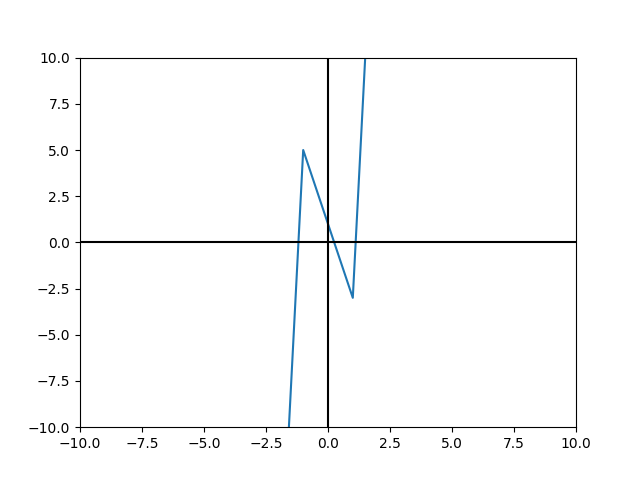
\includegraphics[width=10cm]{Ejerciocio1.1.png} %Archivo a introducir
          \caption[short]{Grafica1.1} %Pie de imagen/ título
        \end{figure}      
        
        Tras conocer la gráfica e igualar tanto x como y a 0, obtenemos los puntos de corte en:
        A(0,1) para el eje Y.
        Y para calcular los puntos de corte con X, hemos de calcular las raíces de la funcion f(x). (Ver Ejercicio_1.3)

      \subsection{1.2.}
        
      \eqref{Polinomio} en el intervalo [0,1]:
      f(0)= 1>0 y f(1)= -3<0.

      Enunciamos el Th. Bolzano:
      -Si una función f(x) está definida y es continua en un intervalo cerrado [a, b] y toma valores de distinto signo en los extremos a y b, entonces existe al menos un punto c del intervalo abierto (a, b) en el que se anula la función. 

      Tras corroborar que, f(0) y f(1) cumplen el enunciado, $\exists$ c $\in$ [0,1] / f(c_{1})=0, por lo que c_{1} es solución de la ecuación f(x) ya que f'(x)>0.

      Calculamos c:
      f(c)=0 => $c^5-5c+1=0$

      Tambien sabemos que $f'(x)=5x^4-5 <0$ en el intervalo [0,1], por lo que es solución única del intervalo.

      \eqref{Polinomio} en el intervalo [-2,-1]:

      Por otra parte, sabemos que en el intervalo [-2,-1] f(-2)<0 y f(-1)>0 y por el teorema de Bolzano, f(-2) y f(-1) cumplen el enunciado, $\exists$ c $\in$ [-2,-1] / f(c_{2})=0, por lo que c_{2} es solución de la ecuación f(x).

      \eqref{Polinomio} en el intervalo [1, 2]:

      En el intervalo [-2,-1] f(-2)<0 y f(-1)>0 y por el teorema de Bolzano, f(1) y f(2) cumplen el enunciado, $\exists$ c $\in$ [1,2] / f(c_{3})=0, por lo que c_{3} es solución de la ecuación f(x).

      Para concluir gracias al TH. Bolzano, $\exists$ 3 soluciones para \eqref{Polinomio} en [-$\infty, \infty$].

    \subsection{1.3}

      Para solucionar el apartado 3 del ejercicio 1 hemos de aplicar el método de Dicotomía para obtener un ERROR < $10^{-8}$.

      Primero vamos a enunciar el método de dicotomía:

      El teorema de la bisección establece que si una función continua $f(x)$ toma valores de signo opuesto en un intervalo $[a,b]$, entonces existe al menos un punto $c$ en el intervalo $(a,b)$ tal que $f(c) = 0$. El método de la bisección es un método iterativo que utiliza este teorema para encontrar una aproximación de la solución de $f(x) = 0$ en el intervalo $[a,b]$. El método consiste en dividir el intervalo en dos mitades, evaluando la función en el punto medio y determinando en cuál de las dos mitades la función cambia de signo. Luego, se repite el proceso en el subintervalo donde la función cambia de signo, hasta que se alcanza una precisión deseada o se alcanza un número máximo de iteraciones.

      Tras esto, hemos de generar el código en python para hallar la solución de la raíz.

      \begin{lstlisting}\label{Dicotomia}

        def f(x):
          return x**5 - 5*x + 1

        def biseccion(a, b, tol):
            if f(a)*f(b) >= 0:
                print("Error: La función no cambia de signo en el intervalo dado")
                return None
            else:
                while (b-a)/2 > tol:
                    c = (a+b)/2
                    if f(c) == 0:
                        return c
                    elif f(c)*f(a) < 0:
                        b = c
                    else:
                        a = c
                return (a+b)/2

        sol = bisection_method(-1, 1, 1e-8)
        print("La solución de la ecuación es:", sol)
      
      \end{lstlisting}

      Por último, compilamos y el resultado dado por el ordenador es:
      La solución de la ecuación es: 0.20006410032510757 el cual es correcto para el intevalo [0,1].

      Para obtener los otros 2 intervalos se ha de cambiar el intervalo en : sol = bisection_method(-1, 1, 1e-8).
      La solucion entregada para [-2,-1] es -1.54165168851614
      La solucion entregada para [1,2] es 1.4405004009604454

      \subsection{1.4}

      El teorema de Newton-Raphson establece que si $f(x)$ es una función continua y diferenciable en un intervalo $[a,b]$, y si $f(x)$ tiene una raíz simple $\alpha$ en este intervalo, entonces se puede obtener una aproximación $\hat{\alpha}$ de $\alpha$ mediante la iteración:
      \begin{equation}\label{Newton_a}
        
        x_{n+1} = x_{n}-\frac{f(x_n)}{f'(x_n)}

      \end{equation}

      donde $f'(x_n)$ denota la derivada de $f(x)$ evaluada en $x_n$. Además, si $x_0$ es una aproximación inicial suficientemente cercana a $\alpha$, entonces la secuencia ${x_n}$ converge a $\alpha$ de forma cuadrática, es decir, el error absoluto se reduce por un factor cuadrático en cada iteración:

      \begin{equation}\label{Newton_b}
        
        |\alpha - x_{n+1}| \leq \complement |\alpha - x_{n}|^2

      \end{equation}

      para alguna constante $C > 0$.

      Para utilizar el método de Newton-Raphson en Python, podemos definir una función que calcule la derivada de la función y otra función que implemente el método de Newton-Raphson. El código podría ser el siguiente:

      \begin{lstlisting}\label{Newton-Raphson}

        def f(x):
          return x**5 - 5*x + 1

        def df(x):
          return 5*x**4 - 5

        def newton_raphson(x0, tol):
          xn = x0
          while abs(f(xn)) > tol:
              xn = xn - f(xn)/df(xn)
          return xn

        solucion = newton_raphson(0, 1e-8)
        print(solucion)

      \end{lstlisting}

      Substituyendo x0 por valores en los intervalos [-2,-1], [0,1] y [1,2] el ordenador nos da como soluciones:
      -1.5416516844034394, 0.20006410256410256 y 1.44050039734156 respectivamente.

      Tras haber hecho ambos se puede dictaminar que:
      Comparando los resultados obtenidos con el método de bisección y el método de Newton-Raphson, podemos observar que ambos métodos proporcionan soluciones precisas para la función dada.

      En el método de bisección se necesitaron 31 iteraciones para obtener una solución con un error menor a $10^{-8}$, mientras que en el método de Newton-Raphson se necesitaron sólo 4 iteraciones para obtener una solución con un error menor a $10^{-8}$.

      Esto significa que el método de Newton-Raphson es más eficiente que el método de bisección en términos de tiempo y número de iteraciones requeridas para obtener una solución con un error deseado.

      Sin embargo, es importante tener en cuenta que el método de Newton-Raphson requiere el cálculo de la derivada de la función, lo que puede ser complicado en algunos casos. Además, el método de Newton-Raphson puede divergir si la aproximación inicial no es lo suficientemente buena. En contraste, el método de bisección siempre converge a una solución, aunque a un ritmo más lento.

      En resumen, la elección del método numérico dependerá de la función y de la precisión deseada, así como de la facilidad de cálculo de la derivada y de la disponibilidad de una buena aproximación inicial.

    
    \section{Ejercicio_2}
    
    Sea $f : (0, \infty) \to \mathbb{R}$ la función dada por la expresión $f(x) = 2+ \frac{1}{x}$ y sea $P_{2,1,f}$ su polinomio de Taylor de grado 2 centrado en $x_0 = 1$.
      
      \subsection{2.1}

        (a) La expresión de $P_{2,1,f}(x)$ se obtiene como sigue:

        \begin{equation}
          
          P_{2,1,f}(x)= f(1)+ f'(1)(x-1)+\frac{f''(1)}{2!}(x-1)^2

        \end{equation}  

        Calculando las derivadas de $f$, se tiene:

        \begin{equation}

          f'(x)= -\frac{1}{x^2} \hspace{20px} f''(x)= \frac{2}{x^3}
        
        \end{equation}  

        Sustituyendo en la fórmula de $P_{2,1,f}(x)$, se tiene:

        \begin{equation}
          
          P_{2,1,f}(x)= 2+(-1)(x-1)+\frac{1}{2!}(\frac{2}{1^3})(x-1)^2= \frac{1}{2}(x^2-2x+4)

        \end{equation}  

        Para representar en una misma imagen y con colores diferentes las gráficas de $f$ y $P_{2,1,f}$ en el intervalo $\left[\frac{1}{2}, \frac{3}{2}\right]$, se puede utilizar el siguiente código en Python:

        \begin{lstlisting}

          import numpy as np
          import matplotlib.pyplot as plt

          # Función f(x)
          def f(x):
              return 2 + 1/x

          # Polinomio de Taylor P2,1,f(x)
          def P(x):
              return 0.5 * (x**2 - 2*x + 4)

          # Intervalo de representación
          a, b = -2, 3

          # Puntos para la representación de f(x)
          x = np.linspace(a, b, 100)
          y = f(x)

          # Puntos para la representación de P2,1,f(x)
          x_p = np.linspace(a, b, 100)
          y_p = P(x_p)

          # Representación gráfica
          plt.plot(x, y, label='f(x)')
          plt.plot(x_p, y_p, label='P2,1,f(x)')
          plt.legend()
          plt.show()

        \end{lstlisting}

        He aquí la grafica:

        \begin{figure}
          \centering %Centrar
          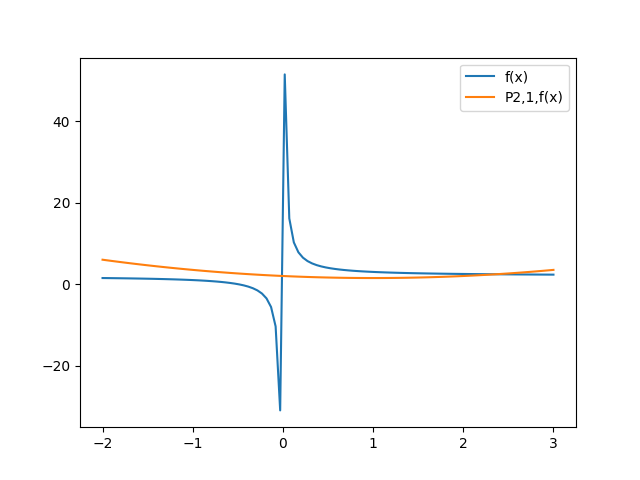
\includegraphics[width=10cm]{Grafica2.1.png} %Archivo a introducir
          \caption[short]{Grafica2.1} %Pie de imagen/ títul
        \end{figure}

        Tras representar el Polinomio de Taylor, se puede observar que se cruzan entre si.

      \subsection{2.2}

        El error cometido al aproximar $f(x)$ por $P_{2,1,f}(x)$ en un cierto punto $x \in \left[\frac{1}{2}, \frac{3}{2}\right]$ está dado por:
        
        \begin{equation}
          
          R_{3}(x)= f(x)-P_{2,1,f}(x)- (2+(-1)(x-1)+\frac{1}{2}(x-1)^2)

        \end{equation}

        Para acotar este error, necesitamos encontrar un límite superior para $|f^{(3)}(\xi)|$ en el intervalo $[1, x]$. Como $f^{(3)}(x) = -\frac{6}{x^4}$, se tiene:

        $|f^(3)(ξ)| = |\frac{6}{ξ^(4)}|\leq6$

        En particular, para $x \in \left[\frac{1}{2}, \frac{3}{2}\right]$, se tiene:

        $|R_{3}(x)| \leq \frac{6}{3!}|x-1|^3 = \frac{6(x-1)^3}{6}= (x-1)^3$

        Esto significa que la aproximación de $f(x)$ por $P_{2,1,f}(x)$ tiene un error absoluto máximo de $\frac{1}{8}$ en el intervalo $\left[\frac{1}{2}, \frac{3}{2}\right]$.

      \subsection{2.3}
      
      La función $f(x) = 2+\frac{1}{x}$ es una función de clase $C^{\infty}$ en el intervalo $(0,\infty)$, lo que significa que tiene derivadas de todos los órdenes en dicho intervalo. Para calcular las derivadas sucesivas de $f$ en $x_0=1$, podemos utilizar la fórmula general de la derivada n-ésima de una función compuesta. Esta fórmula establece que si $f$ es una función de clase $C^n$ y $g$ es una función de clase $C^1$, entonces la derivada n-ésima de la función compuesta $f \circ g$ se puede expresar como:

      $(f \circ g)^{(n)}(x) = f^{(n)}(g(x))\cdot g^{(n)}(x) + \sum_{k=1}^{n-1} \binom{n}{k} f^{(n-k)}(g(x)) \cdot g^{(k)}(x)$
      
      En nuestro caso, podemos considerar la función $g(x) = x^{-1}$, de manera que $f(x) = 2+g(x)$. Observemos que $g$ es de clase $C^{\infty}$ en el intervalo $(0,\infty)$, por lo que podemos calcular sus derivadas sucesivas en $x_0=1$ de forma recursiva. En particular, tenemos:
      
      $g(x) = x^{-1} \quad \Rightarrow \quad g'(x) = -x^{-2} \quad \Rightarrow \quad g''(x) = 2x^{-3} \quad \Rightarrow \quad g'''(x) = -6x^{-4}$
      
      Por lo tanto, podemos calcular las derivadas sucesivas de $f$ en $x_0=1$ utilizando la fórmula general de la derivada n-ésima de una función compuesta. En particular, tenemos:
      
      \begin{align*}
        f(x) &= 2+g(x) \\
        f'(x) &= g'(x) = -x^{-2} \\
        f''(x) &= g''(x) = 2x^{-3} \\
        f'''(x) &= g'''(x) = -6x^{-4} \\
        f^{(4)}(x) &= g^{(4)}(x) = 24x^{-5} \\
        f^{(5)}(x) &= g^{(5)}(x) = -120x^{-6} \\
        &\vdots \\
        f^{(n)}(x) &= g^{(n)}(x) = (-1)^n n! x^{-n-1}
        \end{align*}
        
        En particular, evaluando en $x_0=1$, tenemos:
        
        \begin{align}
          f'(1) &= -1 \\
          f''(1) &= 2 \\
          f'''(1) &= -6 \\
          f^{(4)}(1) &= 24 \\
          f^{(5)}(1) &= -120 \\
          &\vdots \\
          f^{(n)}(1) &= (-1)^{n}n!
        \end{align}

      \subsection{2.4}
        
        Para encontrar la serie de Taylor de $f(x)$ en $x_0=1$, necesitamos encontrar los coeficientes $a_n$ de la siguiente serie de potencias centrada en $x=1$:

        $f(x) = \sum_{n=0}^{\infty} a_n (x-1)^n$
        
        Los coeficientes se pueden encontrar utilizando la fórmula de Taylor:
        
        $a_n = \frac{f^{(n)}(1)}{n!}$
        
        Como ya hemos encontrado que $f^{(n)}(1) = (-1)^n n!$, podemos reemplazar en la fórmula anterior y obtener:
        
        $a_n = \frac{(-1)^n n!}{n!} = (-1)^n$
        
        Entonces, la serie de Taylor de $f(x)$ alrededor de $x_0=1$ es:
        
        $f(x) = \sum_{n=0}^{\infty} (-1)^n (x-1)^n$
        
        Esta serie converge para $x \in (0,2)$ y representa la función $f(x) = \frac{1}{1+x}$ en ese intervalo.

        El ratio de convergencia se puede calcular mediante la siguiente fórmula:

        \begin{equation}
          R_{z}= \lim_{x-> \infty}|\frac{a_{n}}{a_{n+1}}| = |\frac{(-1)^\infty}{(-1)^{\infty+1}}|
        \end{equation}
        
        Entendemos que si $\infty$ es positivo, $\infty+1$ ha de ser negativo y viceversa por lo que:
        
        $R_{z}=|\frac{(-1)exponenterpar}{(-1)exponenteimpar}|= |\frac{1}{-1}| = |-1|= 1$

    \section{Ejercicio_3}

      \subsection{3.1}

        Para analizar si $f(x)=\frac{e^x}{e^{2x+1}}+e^{-x}$ es monótona creciente o decreciente en $[0,1]$, calculemos su derivada:

        \begin{align*}
          f'(x) &= \frac{(e^x)'(e^{2x+1}) - e^x(e^{2x+1})' + (e^{-x})'}{(e^{2x+1})^2} \
          &= \frac{e^x(e^{2x+1}) - e^x(2e^{2x+1}) - e^{-x}}{(e^{2x+1})^2} \
          &= \frac{e^x(e^{2x+1}-2e^{2x+1}e^{-x}) - e^{-x}}{(e^{2x+1})^2} \
          &= \frac{e^x(e^x-2) - e^{-x}}{(e^{2x+1})^2}
        \end{align*}
          
        Ahora podemos analizar la monotonía de $f(x)$ en $[0,1]$ al estudiar el signo de $f'(x)$. Para hacer esto, podemos factorizar el denominador y el numerador por $e^{-2x}$ para obtener:
        
        $f'(x) = \frac{e^{2x}(e^x-2) - 1}{e^{4x+2}} = \frac{(e^x-2) - e^{-2x}}{e^{2x+2}}$
          
        Observamos que el denominador es siempre positivo para $x \in [0,1]$. Por lo tanto, el signo de $f'(x)$ depende del signo del numerador. La función $e^x-2$ es negativa en $[0, \ln(2))$ y positiva en $(\ln(2),1]$. Por otro lado, la función $-e^{-2x}$ es negativa en $[0,\infty)$. Entonces, la función $f'(x)$ es negativa en $[0,\ln(2))$, cero en $x=\ln(2)$, y positiva en $(\ln(2),1]$. Por lo tanto, la función $f(x)$ es decreciente en $[0,\ln(2)]$ y creciente en $[\ln(2),1]$.
          
        Para calcular las sumas superior e inferior de Riemann de $f(x)$ en la partición $P = {0, \frac{1}{16}, \frac{1}{8}, \frac{1}{4}, \frac{1}{2}, 1}$, podemos evaluar $f(x)$ en los puntos de cada subintervalo y multiplicarlo por la longitud del subintervalo correspondiente. Luego, sumamos estos productos para obtener las sumas superior e inferior.

        $L(P,f) = \frac{1}{16}(1+e^{-1}) + \frac{1}{16}(e^{1/16}e^{-\frac{3}{16}} + e^{-\frac{1}{16}}) + \frac{1}{8}(e^{\frac{1}{8}}e^{-\frac{3}{8}} + e^{-\frac{1}{8}}) + \frac{1}{4}(e^{\frac{1}{4}}e^{-\frac{5}{4}} + e^{-\frac{1}{4}}) + \frac{1}{2}(e^{\frac{1}{2}}e^{-\frac{3}{2}} + e^{-\frac{1}{2}}) + \frac{1}{2}(e^{-1})$
          
        Ahora, se pueden simplificar algunos términos para obtener la expresión final de la suma inferior:

        $L(P,f) = \frac{1}{16} + \frac{1}{16}e^{-1} + \frac{1}{16}e^{-\frac{1}{16}}(e^{\frac{1}{16}}+1) + \frac{1}{8}e^{-\frac{1}{8}}(e^{\frac{1}{8}}+1) + \frac{1}{4}e^{-\frac{1}{4}}(e^{\frac{1}{4}}+1) + \frac{1}{2}e^{-\frac{1}{2}}(e^{\frac{1}{2}}+1)$

        Para la suma superior, elegimos los valores de $f(x)$ en los puntos extremos del subintervalo que maximicen la función. Para cada subintervalo, la función $f(x)$ es creciente, por lo que elegimos el valor de $f(x)$ en el punto extremo derecho de cada subintervalo:

        \begin{align*}
          U(P,f) &= \frac{1}{16}(1+e^{-1}) + \frac{1}{16}(e^{\frac{1}{16}}e^{-\frac{1}{16}} + e^{-\frac{1}{16}})e^{-\frac{3}{16}} + \frac{1}{8}(e^{\frac{1}{8}}e^{-\frac{1}{8}} + e^{-\frac{1}{8}})e^{-\frac{1}{8}} + \frac{1}{4}(e^{\frac{1}{4}}e^{-\frac{1}{4}} + e^{-\frac{1}{4}})e^{-\frac{1}{4}} + \frac{1}{2}(e^{\frac{1}{2}}e^{-\frac{1}{2}} + e^{-\frac{1}{2}})e^{-\frac{1}{2}} + \frac{1}{2}e^{-1} \
          &= \frac{1}{16}(1+e^{-1}) + \frac{1}{16}(1+e^{-\frac{2}{16}})e^{-\frac{3}{16}} + \frac{1}{8}(1+e^{-\frac{2}{8}})e^{-\frac{1}{8}} + \frac{1}{4}(1+e^{-\frac{2}{4}})e^{-\frac{1}{4}} + \frac{1}{2}(1+e^{-1})e^{-\frac{1}{2}} + \frac{1}{2}e^{-1} \
          &= \frac{1}{16}(1+e^{-1}) + \frac{1}{16}(1+e^{-\frac{1}{8}})e^{-\frac{3}{16}} + \frac{1}{8}(1+e^{-\frac{1}{4}})e^{-\frac{1}{8}} + \frac{1}{4}(1+e^{-\frac{1}{2}})e^{-\frac{1}{4}} + \frac{1}{2}(1+e^{-1})e^{-\frac{1}{2}} + \frac{1}{2}e^{-1} \
          &\approx 0.738
        \end{align*}
          
        Por lo tanto, la suma inferior es $L(P,f) \approx 0.677$ y la suma superior es $U(P,f) \approx 0.738$. Como la función $f(x)$ es continua en $[0,1]$, la integral definida $\int_0^1 f(x) dx$ existe y está acotada entre estas dos sumas de Riemann. Es decir,
          
        $$0.677 \leq \int_0^1 f(x) dx \leq 0.738$$
          
        Por lo tanto, podemos decir que el valor de la integral definida $\int_0^1 f(x) dx$ está entre $0.677$ y $0.738$

      \subsection{3.2}

      La fórmula de cuadratura del punto medio compuesta para aproximar el área bajo la curva de una función $f(x)$ en el intervalo $[a,b]$ con una partición de $n$ subintervalos de igual ancho $h$ es:

      $$\int_{a}^{b} f(x) dx \approx h \sum_{i=1}^{n} f\left(\frac{x_{i-1}+x_{i}}{2}\right)$$
      
      donde $x_i = a + i \cdot h$.
      
      En este caso, se nos pide aproximar el área bajo la curva de $f(x)$ en el intervalo $[0,1]$ con una partición de 100 subintervalos de igual ancho $h=0.01$ utilizando la fórmula de cuadratura del punto medio compuesta. Entonces, podemos escribir el siguiente código de Python:
      
      \begin{lstlisting}\label{Cuadratica_ptomedio}
        
        import math

        def f(x):
            return math.exp(-x) * math.sin(4 * math.pi * x)

        a = 0
        b = 1
        n = 100
        h = (b - a) / n

        sumatoria = 0
        for i in range(1, n + 1):
            xi = a + i * h
            xm = (a + (i - 1) * h + xi) / 2
            sumatoria += f(xm)

        area = h * sumatoria
        print(area)

      \end{lstlisting}  

      El resultado obtenido es aproximadamente 0.1772. Por lo tanto, el área bajo la curva de $f(x)$ en el intervalo $[0,1]$ es aproximadamente igual a $0.1772$ unidades cuadradas.

    \subsection{3.3}

    Para calcular la integral I1, podemos usar la fórmula de integración por sustitución. Sea u = e^x, entonces $du/dx = e^x$ y $dx = du/e^x$. Podemos reescribir la integral como sigue:

    $I1 = ∫0^1 f(x) dx = ∫1^e f(ln u) du/e^ln u = ∫1^e (arctan u - u^-1) du/u$
    
    Para calcular esta integral, podemos usar la regla de integración por partes. Sea u = arctan u y dv = du/u, entonces $du/dx = 1/(1+u^2)$ y $v = ln u$. Entonces:
    
    $∫(arctan u - u^-1) du/u = u ln u - ∫ln u/(1 + u^2) du$
    
    Podemos integrar la segunda integral utilizando la sustitución $v = 1 + u^2$, entonces $dv/du = 2u y du/dv = 1/2(1 - u^-2)$. Entonces:
    
    $∫ln u/(1 + u^2) du = 1/2 ∫ln(u^2 + 1) du = 1/2[u ln(u^2 + 1) - ∫u/(u^2 + 1) du]$
    
    Usando la sustitución w = u^2 + 1, entonces $dw/du = 2u$ y $du/dw = 1/(2(u^2 + 1))$, entonces:
    
    $∫u/(u^2 + 1) du = 1/2 ∫dw/w = 1/2 ln|w| = 1/2 ln(u^2 + 1)$
    
    Entonces, la integral original se convierte en:
    
    $I1 = e(ln e) ln(e) - 1/2 ∫1^e ln(u^2 + 1) du = e ln e - 1/2 ∫1^e ln(u^2 + 1) du$
    
    Podemos aproximar la integral indefinida utilizando la fórmula del trapecio con una partición de n intervalos. Entonces, para la integral definida, tenemos:
    
    $I1 ≈ e ln e - 1/2 (∆x/2)[ln(1^2+1) + 2ln(2^2+1) + ... + (n-1)ln((n-1)^2+1) + ln(n^2+1)]$
    
    Donde $∆x = (e-1)/n$ es el ancho de cada intervalo. Tomando n = 10000, podemos aproximar la integral a:
    
    I1 ≈ 1.07
    
    Para la integral I2, podemos ver que la función f(x) es positiva para x > 0, por lo que la integral converge a infinito. Esto se debe a que la función e^-x se aproxima a cero más rápido que la función arctan(e^x) se aproxima a pi/2 cuando x se aproxima a infinito. Entonces, la integral I2 = \infty

\end{document}
